\chapter{My Second Chapter}
\ifpdf
    \graphicspath{{Chapter2/Chapter2Figs/PNG/}{Chapter2/Chapter2Figs/PDF/}{Chapter2/Chapter2Figs/}}
\else
    \graphicspath{{Chapter2/Chapter2Figs/EPS/}{Chapter2/Chapter2Figs/}}
\fi

\markboth{\MakeUppercase{\thechapter. My Second Chapter }}{\thechapter. My Second Chapter}


\section{Some Standard things that you may need}

\subsection{Tables}

This subsection contains a few examples of tables such as table \ref{tab:TestTable} and table \ref{tab:StatusData}.  It also shows a use case for the tabularx environment shown in table \ref{tab:tabularx}.\\


\begin{table}[ht]
	\centering
	\begin{tabular}{|c|c|}
		\hline
		Item & Entry \\
		\hline
		Item  & Entry \\
		\hline
	\end{tabular}
	\caption{Table Name}
	\label{tab:TestTable}
\end{table}

\begin{table}[ht]
	\begin{tabularx}{\textwidth}{ |X|X| }
		\hline
		\textbf{Important stuff:} & As stated \\
		\hline 
		\textbf{More Important Stuff:}  & As stated  \\
		\hline
	
	\end{tabularx}
	\caption{tab:Using TabularX}
	\label{tab:tabularx}
\end{table}

\begin{table}[ht]
	\centering
	\begin{tabular}{ |c|r| }
		\hline
		\textbf{No.} & \textbf{Status Data} \\
		\hline 
		1 &  Some \\ 
		2 &  Data \\ 
		3 &  shown\\ 
		4 &  here \\
		\hline
	\end{tabular}
	\caption{Status Data}	
	\label{tab:StatusData}
\end{table}


\subsection{Figures}

Generally, images are pretty simple.  Use .jpg or png and you will be fine.  Just remember the captions.  If you need to rotate an image, you will have to do slightly more work.  All images here are licences under Creative Commons.

% TODO: \usepackage{graphicx} required
\begin{figure}[ht]
	\centering
	\includegraphics[width=0.7\linewidth]{./jpg/ColorfullSky.jpg}
	\caption[Colorfull Sky]{Colorful clouds and blue sky with water reflection of an island hosting trees at sunrise in Si Phan Don, Laos. Basile Morin, CC BY-SA 4.0}
	\label{fig:ColorSky}
\end{figure}


\begin{sidewaysfigure}[ht]
	\centering
	\includegraphics[width=1.0\linewidth]{./jpg/ColorfullSky.jpg}
	\caption{Sideways Image}
	\label{fig:SidewaysImage}
\end{sidewaysfigure}


\subsection{Vector Graphic Images}
Vector graphics can be handled in two ways.  Firstly, you can use eps files generated in another application, or secondly you can create the images on the fly using tikzpicture. A vector image is shown in figure \ref{fig:VennDiagram}.

\begin{figure}[ht]
	\centering
	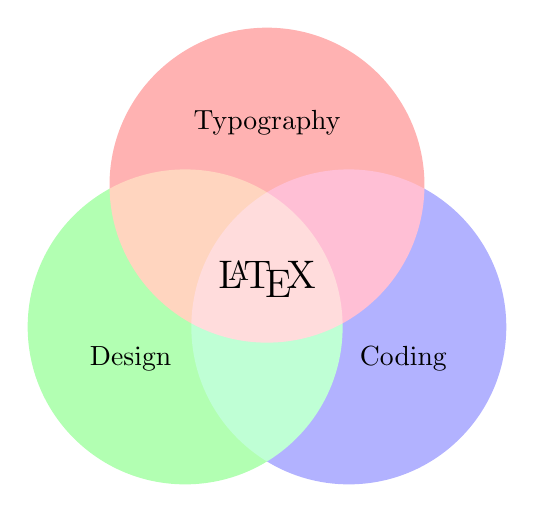
\begin{tikzpicture}
		\begin{scope}[blend group = soft light]
			\fill[red!30!white]   ( 90:1.2) circle (2);
			\fill[green!30!white] (210:1.2) circle (2);
			\fill[blue!30!white]  (330:1.2) circle (2);
		\end{scope}
		\node at ( 90:2)    {Typography};
		\node at ( 210:2)   {Design};
		\node at ( 330:2)   {Coding};
		\node [font=\Large] {\LaTeX};
	\end{tikzpicture}
	\label{fig:VennDiagram}
	\caption{More Vector examples from: \href{https://texample.net/tikz/examples/all/}{https://texample.net/tikz/examples/all/}}
\end{figure}

\newpage
\section{Computer Code}

\subsection{No Code Highlighting}
There are a few useful options for code also.  If you just want a simple listing, without code highlighting, then 'verbatium' is a good option.  You will have to convert tabs to 4 spaces.
\begin{verbatim}
def scope_test():
    def do_local():
        spam = "local spam"
	
    def do_nonlocal():
        nonlocal spam
        spam = "nonlocal spam"
	
    def do_global():
        global spam
        spam = "global spam"
	
    spam = "test spam"
    do_local()
    print("After local assignment:", spam)
    do_nonlocal()
    print("After nonlocal assignment:", spam)
    do_global()
    print("After global assignment:", spam)
	
    scope_test()
    print("In global scope:", spam)
\end{verbatim}


\subsection{Code Highlighting}

The Listings package will add code highlighting for you, but will not add color. The example shown is for Python; this can be changed to other languages by setting the language correctly.


\begin{lstlisting}[language=Python]
	import numpy as np
	
	def incmatrix(genl1,genl2):
	m = len(genl1)
	n = len(genl2)
	M = None #to become the incidence matrix
	VT = np.zeros((n*m,1), int)  #dummy variable
	
	#compute the bitwise xor matrix
	M1 = bitxormatrix(genl1)
	M2 = np.triu(bitxormatrix(genl2),1) 
	
	for i in range(m-1):
	for j in range(i+1, m):
	[r,c] = np.where(M2 == M1[i,j])
	for k in range(len(r)):
	VT[(i)*n + r[k]] = 1;
	VT[(i)*n + c[k]] = 1;
	VT[(j)*n + r[k]] = 1;
	VT[(j)*n + c[k]] = 1;
	
	if M is None:
	M = np.copy(VT)
	else:
	M = np.concatenate((M, VT), 1)
	
	VT = np.zeros((n*m,1), int)
	
	return M
\end{lstlisting}

The lstlisting environment can be customised to show color syntax highlighting, but it takes a bit of work and is specific to the language.  A good tutorial is here \href{https://denbeke.be/blog/programming/syntax-highlighting-in-latex/}{https://denbeke.be/blog/programming/syntax-highlighting-in-latex/}


